\documentclass[12pt]{article}

%figure
\usepackage{booktabs}
\usepackage{graphicx}
\graphicspath{ {fig/} }
\usepackage{caption}

%colors
\usepackage{xcolor}
\definecolor{codegreen}{rgb}{0,0.6,0}
\definecolor{codegray}{rgb}{0.5,0.5,0.5}
\definecolor{codepurple}{rgb}{0.58,0,0.82}
\definecolor{backcolour}{rgb}{0.95,0.95,0.92}

%listings
\usepackage{listings}
\lstloadlanguages{[11]C++}
\lstset{defaultdialect=[11]C++}
\lstset{escapeinside={(*@}{@*)}}

\lstdefinestyle{mystyle}{
    language=C++,
    backgroundcolor=\color{backcolour},   
    commentstyle=\color{codegreen},
    keywordstyle=\color{magenta},
    numberstyle=\tiny\color{codegray},
    stringstyle=\color{codepurple},
    breakatwhitespace=false,         
    breaklines=true,                 
    captionpos=b,                    
    keepspaces=true,                
    numbers=left,                    
    numbersep=5pt, %3pt
    numberstyle=\tiny,
    showlines=true,               
    showspaces=false,                
    showstringspaces=false,
    showtabs=false,                  
    tabsize=2,
    columns=flexible,
    mathescape=true,
    morekeywords={}
}

\lstdefinestyle{myinlinestyle}{
  language=C++,
  backgroundcolor=\color{backcolour},  
  commentstyle=\color{codegreen},
  keywordstyle=\color{magenta},
  stringstyle=\color{codepurple},
  breakatwhitespace=false,         
  keepspaces=true,                
  showspaces=false,                
  showstringspaces=false,
  showtabs=false,                  
  tabsize=2,
  columns=flexible,
  mathescape=true,
  morekeywords={}
}
\newcommand{\ilist}[1]{\lstinline[style=myinlinestyle,basicstyle=\ttfamily,]{#1}}

\title{\databroker User Guide}
\date{v0.7.0\footnote{Please refer to Doxygen documentation for most
    up-to-date API descriptions. A doxygen config file is provided in
    the doc directory.}}

\begin{document}
\maketitle
\section{\databroker}
\label{sec:interface}

The \databroker (DBR) is a distributed, container of key-value stores
enabling applications in a workflow to exchange data through one or
more shared namespaces.  Thanks to a small set of primitives,
applications in a workflow deployed in a (possibly) shared nothing
distributed cluster, can easily share and exchange data and messages
with a minimum effort. Inspired by the Linda coordination and
communication model, the \databroker provides a unified shared
namespace to applications, which is independent from applications'
programming and communication model.



The \databroker is in charge of creating and managing the underlying
namespaces and providing access to them from the user applications.
Basically, the DBR acts as a middleware between the effective
instantiation of each namespace and the applications at the user level
(i.e., applications in the workflow).  The instantiation of the
namespace is done at the backend level and it depends on the runtime
chosen for that purpose. It can be any key-value store as well as
software-based global address space (see \ref{sec:arch}). This
implementation provides Redis\footnote{https://redis.io/} as backend.

\subsection{Architecture}
\label{sec:arch}
\begin{figure}[!htb]
	\centering
	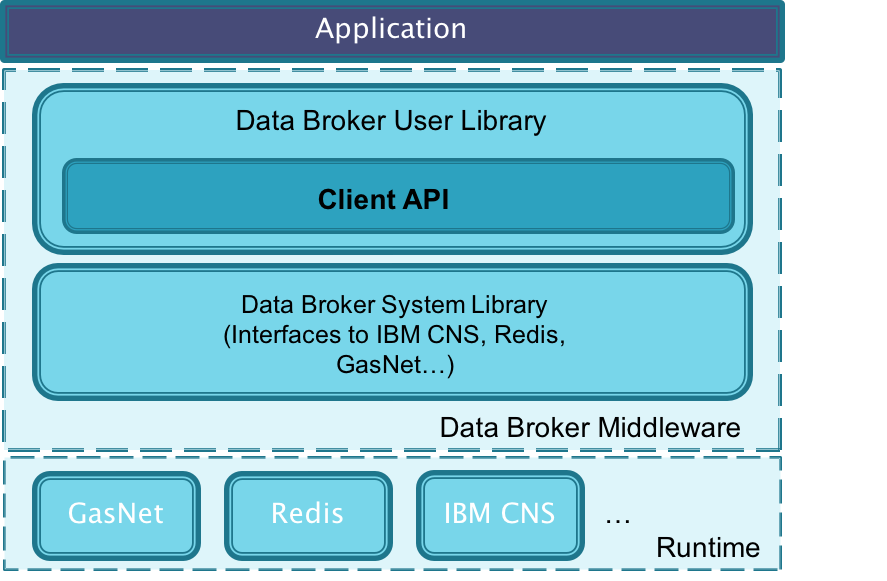
\includegraphics[width=0.7\linewidth]{fig/architecture}
	\caption{Architecture stack of the \databroker.}
	\label{fig:architecture}
\end{figure}


Figure~\ref{fig:architecture} shows a representation of the DBR
architecture stack.  We can identify three main layers acting:
application, middleware and runtime.  At the higher level, the
application represents the software or workflow that will use the DBR
to communicate with other applications or the ones within the workflow
itself.  The middleware layer is composed by two parts: the User
Library and the System Library.  Both are exposed to the user for
different purposes. The User Library provides primitives for accessing
the \databroker and, hence, the namespaces. The System Library can be
used as an interface to implement a new backend.


\section{\databroker API Overview}

A data item that is stored in the \databroker, is called a \emph{tuple}.
A tuple has a name or a key and the tuple data.
Data is organized in so called \emph{namespaces}. That means the same
tuple can be added to different name spaces without any interference.

\begin{figure}[!htb]
	\centering
	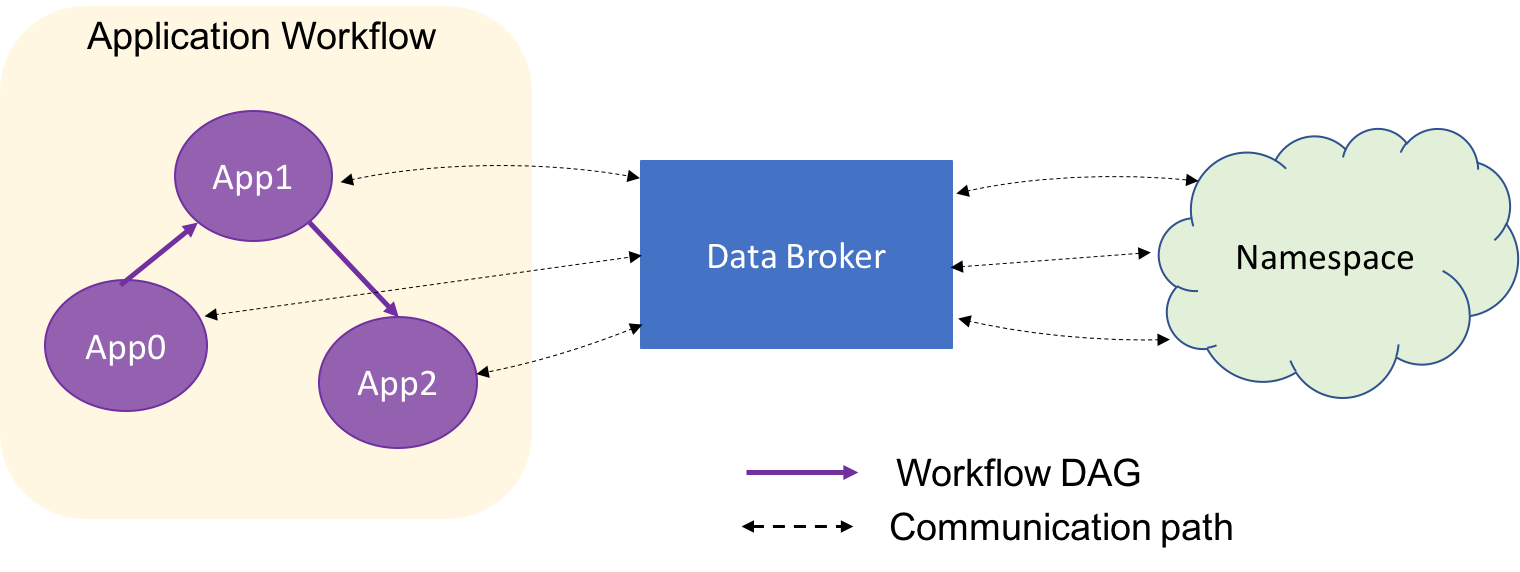
\includegraphics[width=\linewidth]{fig/dbrworkflow}
	\caption{Communication pattern with the \databroker.}
	\label{fig:dbrworkflow}
\end{figure}

Figure~\ref{fig:dbrworkflow} shows the communication pattern among the
three players described: a set of applications send data to the
\databroker, which is in charge of storing such data into the
namespace associated with requests done by applications.


The same tuple (name) can also be added to the same namespace multiple
times, either with the same data or with different data.  In this
case, tuples are pushed into a queue and the insertion order depends
on tuples arrival to the actual storage space (e.\,g.\@ a Redis
server).  Hence, there is no guarantee about the insertion order if
more than one process sends tuples to the same key.  Retrieval of
tuples happens in the order they were stored.  However, again if there
are multiple processes consuming elements from the same queue, it's up
to the processes' coordination to ensure the desired order.




\subsection{Data Access}
\label{sec:interface:access}
\paragraph{Namespace creation} Every access (read or write) to a tuple
requires a valid namespace.  A valid namespace can be either created
(\texttt{dbrCreate()}, code listing~\ref{code:create}) or a process
can attach (\texttt{dbrAttach()}, code listing~\ref{code:attach}) to
an existing namespace.  Namespaces have to be unique, i.\,e.\@ a
namespace creation will fail if there's already an existing namespace
with the same name.

\begin{lstlisting}[style=mystyle,basicstyle=\scriptsize\ttfamily,caption=Creation of a namespace, label=code:create]
int main( int argc, char ** argv )
{
	DBR_Name_t name = strdup("mynamespace");
	DBR_Tuple_persist_level_t level = DBR_PERST_VOLATILE_SIMPLE;
	DBR_GroupList_t groups = 0;
	// create a test name space
	DBR_Handle_t ns_hdl =  dbrCreate(name, level, groups);
	// ...
}
\end{lstlisting}

\begin{lstlisting}[style=mystyle,basicstyle=\scriptsize\ttfamily,caption=Attach to a namespace, label=code:attach]
int main( int argc, char ** argv ) 
{
	DBR_Tuple_persist_level_t level = DBR_PERST_VOLATILE_SIMPLE;
	DBR_GroupList_t groups = 0;
	DBR_Name_t name = strdup("mynamespace");
	
	DBR_State_t ns_state;
	DBR_Handle_t ns_hdl = NULL;
	
	// Check existence of the namespace with the specified name
    ns_hdl = dbrAttach( name );
    if (ret == NULL) {
       // name space doesn't exist or some error happened in the back-end
    } else {
       // successfully attached
    }
		
	// ...
}
\end{lstlisting}

\paragraph{Data insertion} The \texttt{dbrPut} (blocking, listing~\ref{code:put}) and \texttt{dbrPutA}
(non blocking, listing~\ref{code:putA}), allow the user to insert new data to a namespace.  This
requires a valid namespace handle, a tuple name and the pointer and
size of a contiguous memory region containing the tuple data.  The
tuple will be added to the existing namespace and if there's already a
tuple with the same name, the tuple data will be added to that tuple
as a kind of new version of data.
Return values are the following  for \texttt{dbrPut} and \texttt{dbrPutA} respectively:
\begin{itemize}
	\item \texttt{DBR\_Errorcode\_t}: \texttt{ DBR\_SUCCESS} if the put is successful, a \texttt{DBR\_Errorcode\_t} code otherwise (see Table\ref{table:errorcodes}) 
	\item \texttt{DBR\_Tag\_t}: an id of the asynchronous call. It is used to check its completion via \texttt{dbrTest(DBR\_Tag\_t tag)}
\end{itemize}

\begin{lstlisting}[style=mystyle,basicstyle=\scriptsize\ttfamily,caption=Put data into the namespace (blocking), label=code:put]
int main( int argc, char ** argv )
{
	// create or attach to a namespace
	// ...
	
    // Function signature
    // DBR_Errorcode_t dbrPut( DBR_Handle_t ns_handle: handler to the namespace
    // void *va_ptr: buffer containing the data
    // int64_t size: size of the buffer
    // DBR_Tuple_name_t tuple_name: name/key of the value
    // DBR_Group_t group: collection of units of backing memory (not applicable to Redis backend)
    // );
    
    char *in = strdup("Hello World!");
    int64_t in_size = strlen(in);
    DBR_Group_t group = '0';
    
    DBR_Errorcode_t ret = dbrPut(ns_hdl, in, in_size, "testTup", group);
	
	// ...
}
\end{lstlisting}

\begin{lstlisting}[style=mystyle,basicstyle=\scriptsize\ttfamily,caption=Push data to the namespace (non-blocking), label=code:putA]
int main( int argc, char ** argv )
{
	// create or attach to a namespace
	// ...
	
	// Function signature
    //DBR_Tag_t dbrPutA( DBR_Handle_t ns_handle: handler to the namespace
    // void *va_ptr: buffer containing the data
    // int64_t size: size of the buffer
    // DBR_Tuple_name_t tuple_name: name/key of the value
    // DBR_Group_t group: collection of units of backing memory (not applicable to Redis backend)
    // );
    
    char *in = strdup("Hello World!");
    int64_t in_size = strlen(in);	
    DBR_Group_t group = '0';
    
    DBR_Tag_t tag = dbrPutA(ns_hdl, in, in_size, "tuple_key", group);
    if(tag != DBR_TAG_ERROR)
      while ( dbrTest(tag) == DBR_ERR_INPROGRESS );
		
	// ...
}
\end{lstlisting}

\paragraph{Data retrieval} There are 2 types of retrieval functions:
\begin{enumerate}
\item Read without consuming the tuple: the \texttt{dbrRead} (listing~\ref{code:read}) and
  \texttt{dbrReadA} (listing~\ref{code:readA}) APIs retrieve a copy of a tuple of the given name from the
  namespace and will not touch or consume the data.  A read can be
  repeated multiple times without changing the content of the
  namespace.
  The blocking read \texttt{dbrRead} can be customized with two different flags based on the behavior the user prefers:
  \begin{itemize}
  	\item \texttt{DBR\_FLAGS\_NONE}: the call blocks until a certain timeout is reached;
    \item \texttt{DBR\_FLAGS\_NOWAIT}: the call checks whether the tuple exists or not and returns immediately if the tuple is not in the namespace.
  \end{itemize}

Return values are the following  for \texttt{dbrRead} and \texttt{dbrReadA} respectively:
\begin{itemize}
	\item \texttt{DBR\_Errorcode\_t}: \texttt{ DBR\_SUCCESS} if the read is successful, a \texttt{DBR\_Errorcode\_t} code otherwise (see Table~\ref{table:errorcodes}) 
	\item \texttt{DBR\_Tag\_t}: an id of the asynchronous call. It is used to check its completion via \texttt{dbrTest(DBR\_Tag\_t tag)}
\end{itemize}

Furthermore, given the possibility to define the flag to just check wether a tuple exists or not, there will be the possible error codes:
\begin{itemize}
	\item[-] \texttt{DBR\_ERR\_TIMEOUT} if the tuple does not exist \textbf{and} the flag is set to \texttt{DBR\_FLAGS\_NONE} (hence, blocking behaviour);
	\item [-] \texttt{DBR\_ERR\_UNAVAIL} if the tuple does not exist \textbf{and} the flag is set to \texttt{DBR\_FLAGS\_NOWAIT} (hence, immediate return in any case)
\end{itemize}

\begin{lstlisting}[style=mystyle,basicstyle=\scriptsize\ttfamily,caption=Read data from the namespace (blocking), label=code:read]
int main( int argc, char ** argv )
{
	// create or attach to a namespace
	// ...
	
	// Function signature
	// DBR_Errorcode_t dbrRead( DBR_Handle_t ns_handle: handler to the namespace
    //    void *va_ptr: buffer to store received data
    //    int64_t *size: current size of the buffer, this value will be set with the size of received data 
    //    DBR_Tuple_name_t tuple_name: name/key for the tuple to be searched
    //    DBR_Tuple_template_t match_template: template to match for tuple name/key
    //    DBR_Group_t group: collection of units of backing memory (not applicable to Redis backend)
    //    int flags: DBR_FLAGS_NONE, DBR_FLAGS_NOWAIT
    // );
	
	char *recv_buffer = (char*)malloc(1024);
	int64_t buf_size = 1024;
	DBR_Group_t group = '0';
	DBR_Tuple_template_t match_template = "";
    
    memset(recv_buffer, 0, buf_size);
	DBR_Tuple_name_t tuple_key = "some_key";
	DBR_Errorcode_t ret = dbrRead(ns_hdl, recv_buffer, &buf_size, tuple_key, match_template, group, DBR_FLAGS_NONE);
	
	// ...
}
\end{lstlisting}
  
\begin{lstlisting}[style=mystyle,basicstyle=\scriptsize\ttfamily,caption=Read data from the namespace (non-blocking), label=code:readA]
int main( int argc, char ** argv )
{
	// create or attach to a namespace
	// ...

    // Function signature
    //DBR_Tag_t  dbrReadA( DBR_Handle_t ns_handle: handler to the namespace 
    //    void *va_ptr: buffer to store received data
    //    int64_t *size: current size of the buffer, this value will be set with the size of received data 
    //    DBR_Tuple_name_t tuple_name: name/key for the tuple to be searched
    //    DBR_Tuple_template_t match_template: template to match for tuple name/key
    //    DBR_Group_t group: collection of units of backing memory (not applicable to Redis backend)
    // );

	char *recv_buffer = (char*)malloc()1024);
	int64_t buf_size = 1024;
	DBR_Group_t group = '0';
	DBR_Tuple_template_t match_template = "";
	
	memset(recv_buffer, 0, buf_size);
	DBR_Tuple_name_t tuple_key = "some_key";
	DBR_Tag_t tag = dbrReadA(ns_hdl, recv_buffer, &buf_size, tuple_key, match_template, group);
	DBR_Errorcode_t state = 0;
	if( tag != DBR_ERR_TAGERROR)
      while ( dbrTest(tag) == DBR_ERR_INPROGRESS );

	
	// ...
}
\end{lstlisting}


\item Get and consume the tuple: the \texttt{dbrGet} (listing~\ref{code:get}) and \texttt{dbrGetA} (listing~\ref{code:getA}) commands will retrieve and consume a tuple. This means that after a
  get, the tuple will be deleted. Note that only one version of the
  tuple will be removed by a single get call. If there have been
  multiple tuples added with the same name, then the number of
  versions of that tuple is reduced by 1.
The blocking get \texttt{dbrGet} can be customized with two different flags based on the behavior the user prefers:
\begin{itemize}
	\item \texttt{DBR\_FLAGS\_NONE}: the call blocks until a certain timeout is reached;
	\item \texttt{DBR\_FLAGS\_NOWAIT}: the call checks wheter the tuple exists or not and returns immediately if the tuple is not in the namespace.
\end{itemize}

Return values are the following  for \texttt{dbrGet} and \texttt{dbrGetA} respectively:
\begin{itemize}
	\item \texttt{DBR\_Errorcode\_t}: \texttt{ DBR\_SUCCESS} if the read is successful, a \texttt{DBR\_Errorcode\_t} code otherwise (see Table~\ref{table:errorcodes}) 
	\item \texttt{DBR\_Tag\_t}: an id of the asynchronous call. It is used to check its completion via \texttt{dbrTest(DBR\_Tag\_t tag)}
\end{itemize}

Furthermore, given the possibility to define the flag to just check whether a tuple exists or not, there will be the possible error codes:
\begin{itemize}
	\item[-] \texttt{DBR\_ERR\_TIMEOUT} if the tuple does not exist \textbf{and} the flag is set to \texttt{DBR\_FLAGS\_NONE} (hence, blocking behavior);
	\item [-] \texttt{DBR\_ERR\_UNAVAIL} if the tuple does not exist \textbf{and} the flag is set to \texttt{DBR\_FLAGS\_NOWAIT} (hence, immediate return in any case)
\end{itemize}


\begin{lstlisting}[style=mystyle,basicstyle=\scriptsize\ttfamily,caption=Get data from the namespace (blocking), label=code:get]
int main( int argc, char ** argv )
{
	// create or attach to a namespace
	// ...

    // Function signature
    // DBR_Errorcode_t dbrGet( DBR_Handle_t ns_handle: handler to the namespace
    //    void *va_ptr: buffer to store received data
    //    int64_t *size: current size of the buffer, this value will be set with the size of received data 
    //    DBR_Tuple_name_t tuple_name: name/key for the tuple to be searched
    //    DBR_Tuple_template_t match_template: template to match for tuple name/key
    //    DBR_Group_t group: collections of unit of backing memory (not applicable to Redis backend)
    //    int flags: DBR_FLAGS_NONE, DBR_FLAGS_NOWAIT
    // );

	char *recv_buffer = (char*)malloc(1024);
	int64_t buf_size = 1024;
	DBR_Group_t group = '0';
	DBR_Tuple_template_t match_template = "";
	
	memset(recv_buffer, 0, buf_size);
	DBR_Tuple_name_t tuple_key = "some_key";
	DBR_Errorcode_t ret = dbrGet(ns_hdl, recv_buffer, &buf_size, tuple_key, match_template, group, DBR_FLAGS_NOWAIT);
	
	// ...
}
\end{lstlisting}

  \begin{lstlisting}[style=mystyle,basicstyle=\scriptsize\ttfamily,caption=Get data from the namespace (non-blocking), label=code:getA]
int main( int argc, char ** argv )
{
	// create or attach to a namespace
	// ...

    // Function signature
    //DBR_Tag_t  dbrGetA( DBR_Handle_t ns_handle: handler to the namespace 
    //    void *va_ptr: buffer to store received data
    //    int64_t *size: current size of the buffer, this value will be set with the size of received data 
    //    DBR_Tuple_name_t tuple_name: name/key for the tuple to be searched
    //    DBR_Tuple_template_t match_template: template to match for tuple name/key
    //    DBR_Group_t group: collections of unit of backing memory (not applicable to Redis backend)
    // );
	
	char *recv_buffer = (char*)malloc(1024);
	int64_t buf_size = 1024;
	DBR_Group_t group = '0';
	DBR_Tuple_template_t match_template = "";

	memset(recv_buffer, 0, buf_size);
	DBR_Tuple_name_t tuple_key = "some_key";
	DBR_Tag_t tag = dbrReadA( ns_hdl, recv_buffer, &buf_size, tuple_key, match_template, group);
	DBR_Errorcode_t state = 0; 

	if(tag != DBR_ERR_TAGERROR)
      while ( dbrTest(tag) == DBR_ERR_INPROGRESS );
	
	// ...
}
\end{lstlisting}
Both, read and get will return one version of a stored tuple in case
there are more versions available.  If there's no tuple with the
requested name available in the namespace, read (\texttt{dbrRead}) and get (\texttt{dbrGet}) will block
(until a configurable timeout is hit). 
\end{enumerate}


\paragraph{Check existence of a tuple} It is possible to check whether a tuple is present in a namespace or not with the \texttt{dbrTestKey} function (listing~\ref{code:testKey}). It will not return any tuple and does not modify the namespace.

\begin{lstlisting}[style=mystyle,basicstyle=\scriptsize\ttfamily,caption=Check for the existence of a tuple in the \databroker, label=code:testKey]
int main( int argc, char ** argv )
{
// create or attach to a namespace
// ...
// Function signature
// DBR_Errorcode_t dbrTestKey( DBR_Handle_t dbr_handle, DBR_Tuple_name_t tuple_name );
//   DBR_Handle_t dbr_handle: handle to the namespace
//   DBR_Tuple_name_t tuple_name: name/key for the tuple to be searched
// );

	DBR_Errorcode_t ret = dbrTestKey( cs_hdl, "tuple_key" );
// ...
}
\end{lstlisting}

The function will return:
\begin{itemize}
	\item[-] DBR\_SUCCESS if the tuple is present;
	\item[-] DBR\_ERR\_UNAVAIL if the tuple is unavailable;
	\item[-] An error code identifying the issue, otherwise
\end{itemize}




\paragraph{Inventory of keys} is available through the
\texttt{dbrDirectory} API (listing~\ref{code:dbrDirectory}. It
requires a sufficiently sized amount of memory to hold the list of
keys up to an optional limit. The returned list is a comma-separated
sequence of strings representing the available keys. If group is set
to \texttt{DBR\_GROUP\_LOCAL}, the list will only contain tuple names
from a local storage backend.  The determination of what is
\emph{local} depends on the type of backend implementation. For
example the Redis backend would only retrieve data from servers that
run on the same host as the calling process.

\begin{lstlisting}[style=mystyle,basicstyle=\scriptsize\ttfamily,caption=List
  the currently available tuples., label=code:dbrDirectory]
int main( int argc, char ** argv )
{
// create or attach to a namespace
// ...
// Function signature
// DBR_Errorcode_t
// dbrDirectory( DBR_Handle_t cs_handle : handle to the namespace
//               DBR_Tuple_template_t match_template : filter to select only a subset of tuples
//               DBR_Group_t group : storage group to retrieve the keys from
//               const unsigned count : maximum number of entries to retrieve
//               char *result_buffer : memory to hold the list
//               const size_t size : amount of space in that memory
//               int64_t *ret_size : returned number of bytes
// );

	DBR_Errorcode_t ret = dbrDirectory( cs_hdl, "*", DBR_GROUP_EMPTY,
                                        1000, keyspace, keyspace_size,
                                        *nbytes );
// ...
}
\end{lstlisting}


The function will return:
\begin{itemize}
	\item[-] DBR\_SUCCESS if the tuple is present;
	\item[-] An error code identifying the issue, otherwise
\end{itemize}



\paragraph{Iterator} allows to iterate over all or a subset of the
tuples and retrieve the keys one by one.  In comparison to the
inventory, this only requires a small buffer to hold a single key
(which can have a max size of 1024 bytes).

\begin{lstlisting}[style=mystyle,basicstyle=\scriptsize\ttfamily,caption=List
  the currently available tuples., label=code:dbrIterator]
int main( int argc, char ** argv )
{
// create or attach to a namespace
// ...
// Function signature
// DBR_Iterator_t
// dbrIterator( DBR_Handle_t dbr_handle : handle to namespace
//              DBR_Iterator_t it : iterator handle
//              DBR_Group_t group : storage group to iterate
//              DBR_Tuple_template_t match_template : filter to select only a subset of tuples
//              DBR_Tuple_name_t tuple_name : key buffer for returned key
// );

// using iterator input DBR_ITERATOR_NEW to create iterator and return
// first key
// subsequent calls until DBR_ITERATOR_DONE is returned together with
// EOF as the key:

   DBR_Iterator_t it = DBR_ITERATOR_NEW;

   do {
     it = dbrIterator( cs_hdl, it, DBR_GROUP_EMPTY, "*", keyspace );
     if( it != DBR_ITERATOR_DONE )
        // ... do something with the key
   } while( it != DBR_ITERATOR_DONE );
}
\end{lstlisting}

The function will return:
\begin{itemize}
\item [-] An iterator handle which equals \texttt{DBR\_ITERATOR\_DONE}
  if the iterator hits the end of the list of available tuples. If
  this is the case, then the returned key will be \texttt{EOF} or any
  other invalid key.
\end{itemize}


\paragraph{Namespace deletion} Any process that is attached to a
namespace needs to detach \texttt{dbrDetach}
(\ilist{dbrDetach(ns\_hdl);}). The \databroker uses a
reference counter to check how many processes are attached to a
namespace.  Calling \texttt{dbrDelete} (\ilist{dbrDelete(name);}), will check this reference counter
and if it's 0, then the deletion will proceed and clean up all
remaining data of that namespace.



\subsection{Interface Extensions}
\databroker provides a few extensions to the main interface. The main
extension to note here is the ability to work with non-contiguous
tuple data.  \texttt{libdatabroker\_ext.h} needs to be included to
access functions that provide a scatter-gather mechanism for
non-contiguous memory.


\subsection{Example Sequence}
\label{sec:interface:example}
We now show two different scenarios.
If no namespace exists, then:
\begin{enumerate}
\item A process would \texttt{dbrCreate} a new namespace (which
  automatically attaches the process to that namespace too, there's no
  need to do an additional \texttt{dbrAttach})
\item Then the process can put and get data to and from that namespace.
\item At the end, it would call \texttt{dbrDelete} to clean up.
\end{enumerate}

\noindent If a namespace already exists, then:
\begin{enumerate}
\item A process would \texttt{dbrAttach} to an existing namespace.
\item Then the process can put and get data to and from that namespace.
\item At the end, it would call \texttt{dbrDetach} to tell the \databroker
  that no more access to that namespace will occur.
\end{enumerate}

Please see \ref{sec:interface:limits} for current limitations and
problems.

\subsection{Building an Application with the \databroker}
\begin{lstlisting}[basicstyle=\scriptsize\ttfamily,backgroundcolor=\color{backcolour},caption=Example Makefile,captionpos=b,label=code:Makefile]
# Build Environment
CC            = gcc
CXX           = g++
CFLAGS        = -O3
CXXFLAGS      = -O3
INCPATH       = -I./ -I$(DATABROKER_HOME)/include
LINK          = g++ 
LDFLAGS       = -L$(DATABROKER_HOME)/lib
LIBS          = -lstdc++ -ldatabroker -ldbbe_redis
RM            = rm -f
# 
OBJECTS      = single.o
SOURCES      = single.cc
DESTDIR	     = ./
TARGET       = single
#
# Compile
.SUFFIXES: .o .c .cpp .cc .cxx .C
.cpp.o:
    $(CXX) -c $(CXXFLAGS) $(INCPATH) -o "$@" "$<"
.cc.o:
    $(CXX) -c $(CXXFLAGS) $(INCPATH) -o "$@" "$<"
.cxx.o:
    $(CXX) -c $(CXXFLAGS) $(INCPATH) -o "$@" "$<"
.C.o:
    $(CXX) -c $(CXXFLAGS) $(INCPATH) -o "$@" "$<"
.c.o:
    $(CC)  -c $(CFLAGS)   $(INCPATH) -o "$@" "$<"
# 
# Build 
all:  $(TARGET)
$(TARGET): $(OBJECTS) 
    $(LINK) $(LDFLAGS) -o $(TARGET) $(OBJECTS) $(LIBS)
# 
clean:
    $(RM)  $(OBJECTS) $(DESTDIR)/$(TARGET)
\end{lstlisting}

%$
\subsection{Configuration}
\label{sec:interface:config}
There are a few environment variables that can be set by the user to
adjust the behavior of the \databroker library.
\begin{itemize}
\item \texttt{DBR\_SERVER} Points to one of the backend storage
  services in a URL-kind of way. Users specify
  \texttt{<protocol>://<destination>} to select a lookup- and
  connection protocol and a destination.  Currently the only protocol
  is \texttt{sock} and the destination should consist of
  \texttt{<host>:<port>}. If not set, it defaults to
  \texttt{sock://localhost:6379}.  If the backend requires connections
  to multiple servers (for example if Redis runs as a cluster), the
  library will automatically figure out about the locations of the
  other services and restores connections in case of service
  failures+restarts.


\item \texttt{DBR\_AUTHFILE} points to a file that contains the Redis
  authentication password.  The password needs to be in the first line
  of that file. Any further content of that file is ignored. It is
  recommended to use the absolute path when referencing the filename:\\
  \centerline{ \tt export DBR\_AUTHFILE=/path/to/the/authfile.txt}

\item \texttt{DBR\_TIMEOUT} determines the approximate time to wait in
  read or get calls before they fail with a timeout error.

\item \texttt{DBR\_PLUGIN} enables the use of data adapters. The
  variable should point to a shared library file that will be loaded
  by the \databroker library.

\end{itemize}

\subsection{Current Limitations and Problems}
\label{sec:interface:limits}
\begin{enumerate}
\item The namespace reference counting is currently not tracked on a
  per-client basis. That means, a misbehaving process can repeatedly
  detach and decrease the reference count.  Although, that requires a
  modified client library component since the client library also
  checks a process-local reference count.
\item Depending on the backend, there might be a limit on the max size
  of the tuple data.  For example, Redis has a limit of 512MB per data
  item.
\end{enumerate}



\section{Troubleshooting}
\label{sec:interface:troubleshoot}
\subsection{Checking Redis via redis-cli}
\label{sec:interface:troubleshoot:checkredis}
In case things go wrong, Redis comes with a command line client {\tt
  redis-cli}. It's a powerful tool to check the Redis server is
running as expected and also allows to browse and change the content
of the \databroker storage.

The following output is generated by running the command line client
connecting to a Redis server on localhost, then authorizing the access
using the {\tt AUTH} command, and then listing all existing keys on
that server using {\tt KEYS} (showing that there are no keys stored yet:
\begin{lstlisting}[style=mystyle,language=bash,basicstyle=\scriptsize\ttfamily,caption=Redis
  check via command line tool, label=code:rediscli]
> redis-cli -p 6379 -h localhost
localhost:6379> AUTH mysecretpassword
OK
localhost:6379> KEYS *
(empty list or set)
localhost:6379>
\end{lstlisting}

If the server is configured without a password, the {\tt AUTH} command
will return {\tt (error) No authorization required} or a similar
error.
If you enter the wrong password (or the password in the config file
contains unsupported characters like quotes), you'll get an error too.

In case you skip the {\tt AUTH} command and go straight to {\tt KEYS},
you should get an error message similar to: {\tt (error) NOAUTH
  Authentication required}.

\subsection{Cleaning Up}
In case data got stuck in Redis, the command line client {\tt
  redis-cli} can be used to clean up the data. Before doing that, make
sure all clients that use the \databroker library are detached from any
namespace. Otherwise, it might cause inconsistencies between the lib
and the Redis storage.
Start the {\tt redis-cli} and authorize the access (see
\ref{sec:interface:troubleshoot:checkredis}) followed by calling the
Redis command {\tt FLUSHALL}.

\subsection{Connection to Redis failed}
It is important to specify the configuration file when starting a Redis server with the following command \texttt{redis-server <path/to/conf/file>}.
If not specified, the following error will occurr at the application level: 
\begin{lstlisting}[style=mystyle,language=bash,basicstyle=\scriptsize\ttfamily,caption=Connection failed error, label=code:connerr]
dbBE_Redis_context_t::initialize: Failed to connect to Redis.
libdatabroker: failed to create/connect backend.
\end{lstlisting}


\section{Appendix}
\newpage
\subsection{Error Code Table}
\begin {table}[h]
    \scriptsize
\begin{tabular}{l|p{10cm}}
	\toprule
	\textbf{Error Code} & \textbf{Detailed Message} \\
	\toprule
	DBR\_SUCCESS &  No error, clean result, operation successful\\ 
    \midrule
	DBR\_ERR\_GENERIC & A general or unknown error has occurred \\ 
	\midrule
	DBR\_ERR\_INVALID & An invalid parameter was passed into a function or other general error \\ 
	\midrule
	DBR\_ERR\_HANDLE  & An invalid handle was encountered \\
	\midrule
	DBR\_ERR\_INPROGRESS & A request is still in progress, check again later  \\ 
	\midrule
	DBR\_ERR\_TIMEOUT & A timeout occurred  \\ 
	\midrule
	DBR\_ERR\_UBUFFER & Provided user buffer problem (too small, not available)  \\ 
	\midrule
	DBR\_ERR\_UNAVAIL & The requested tuple or namespace is not available in the backing storage \\ 
	\midrule
	DBR\_ERR\_EXISTS & Entry already exists \\ 
	\midrule
	DBR\_ERR\_NSBUSY & There are still clients attached to a namespace \\ 
	\midrule
	DBR\_ERR\_NSINVAL & Invalid name space\\ 
	\midrule
	DBR\_ERR\_NOMEMORY & The amount of memory or storage was insufficient \\ 
	\midrule
	DBR\_ERR\_TAGERROR & The returned tag is an error\\ 
	\midrule
	DBR\_ERR\_NOFILE & A file was not found \\ 
	\midrule
	DBR\_ERR\_NOAUTH & Access authorization required or failed\\ 
	\midrule
	DBR\_ERR\_NOCONNECT & Connection to a storage backend failed  \\ 
	\midrule
	DBR\_ERR\_CANCELLED & Operation was canceled  \\
	\midrule
	DBR\_ERR\_NOTIMPL & Operation not implemented \\ 
	\midrule
	DBR\_ERR\_INVALIDOP & Invalid operation  \\ 
	\midrule
	 DBR\_ERR\_BE\_POST & Posting request to back-end failed  \\ 
	\midrule
	DBR\_ERR\_BE\_GENERAL & Unspecified back-end error \\ 
    \midrule
    DBR\_ERR\_ITERATOR & Invalid iterator or error iterating the namespace \\
    \midrule
    DBR\_ERR\_PLUGIN & Data adapter error \\
    \bottomrule
\end{tabular} 
\caption {List of error codes} 
\label{table:errorcodes} 
\end{table}

\newpage
\subsection{Redis Specifics}

\subsubsection{Connection Management}
The Redis backend maintains connections to a cluster including systems
with Master-Replica configurations.  Connections are not established
to replicas until the corresponding master connection fails. Once that
happens, the library makes an attempt to reconnect to the master and
if that fails, establishes a connection to the replica.  However, if
that replica keeps running as a replica, the library will disconnect
again and try to find the master because only master instances are
allowed to modify data.

\subsubsection{Iterator}
The implementation of the Redis iterator is done in a way to prevent
going to the server for each step of the iteration.  The backend
library caches a number of keys and most requests are served directly
from that cache with immediate completion.  Only if the number of
cached keys drops below a threshold, a new set of keys is retrieved
from Redis.

In case a Redis cluster is used, the list of keys is retrieved from
one server at a time until all keys of that server have been
listed. There's no ordering of keys or servers available. If the set
of keys changes while the iteration is done, there's no guarantee that
a key is still in storage at the time it is returned to the user
because of the cache and because of the way the Redis SCAN command
works.

\end{document}
